\documentclass[aspectratio=169]{beamer}
\usepackage{graphicx}

\title{Deep G-Buffers for stable Global Illumination Approximation}
\author{Ferit Tohidi Far}
\usetheme{Frankfurt}

\begin{document}
	\maketitle

	\begin{frame}
		\frametitle{Content}
		\begin{itemize}
			\item Global illumination
				\begin{itemize}
					\item Pathtracing
					\item Radiosity
					\item Visual effects
					\item Computational difficulty
				\end{itemize}
			\item Traditional rendering
				\begin{itemize}
					\item Forward rendering
					\item Deferred rendering
				\end{itemize}
			\item Deep G-Buffers
				\begin{itemize}
					\item Depth-peeling
					\item Generating a 2-layer deep g-buffer
					\item Global illumination approximation
				\end{itemize}
		\end{itemize}
	\end{frame}

	\begin{frame}
		\frametitle{Global illumination}
		\begin{columns}
			\column{.6\textwidth}
				\begin{itemize}
					\item lighting of a scene
					\item direct \textbf{and indirect} light is considered
					\item causes visual effects that convey realism
					\item $ L_o(\omega) = L_e(\omega) + \int_\Omega f(\omega, \omega')L_i(\omega')cos(n, \omega') \partial \omega' $
					\item most popular method is pathtracing
				\end{itemize}
			\column{.4\textwidth}
				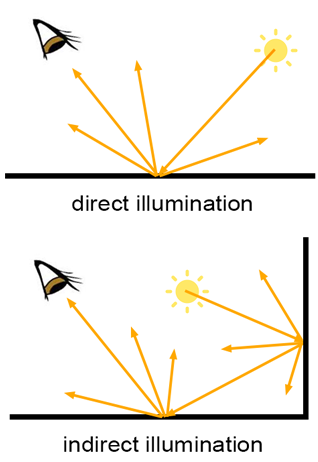
\includegraphics[height=.7\textheight]{img/indirect_illumination.png}
		\end{columns}
	\end{frame}

	\begin{frame}
		\frametitle{Pathtracing}
		\begin{columns}
			\column{.5\textwidth}
				\begin{itemize}
					\item send camera ray through each pixel
					\item allow ray to reflect \textbf{diffusely or specularly}
					\item trace it back to a light source
					\item if a light source was hit, the pixel is colored
					\item else the pixel is black
					\item sample each pixel thousands of times, then average
				\end{itemize}
			\column{.5\textwidth}
				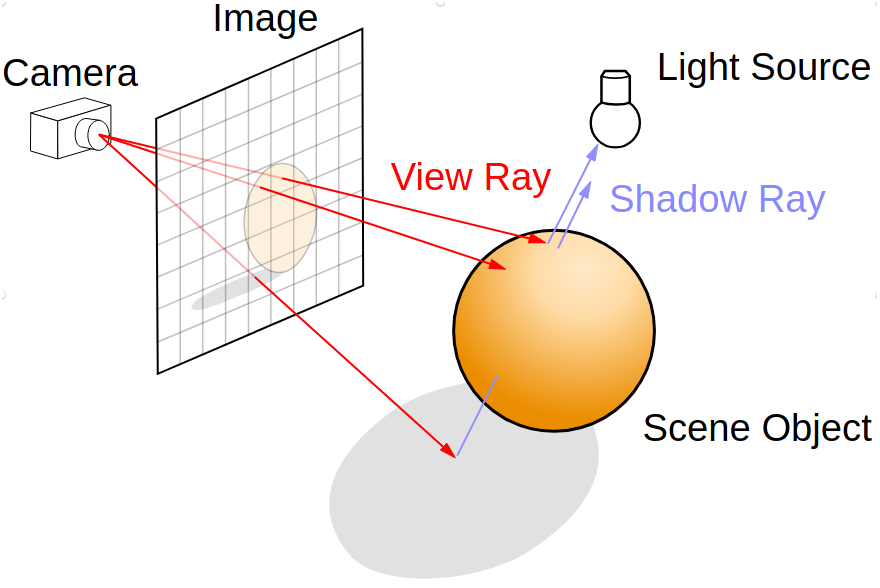
\includegraphics[width=\textwidth]{img/raytrace_tut.png}
		\end{columns}
	\end{frame}

	\begin{frame}
		\frametitle{Radiosity}
		\begin{itemize}
			\item scene is divided into patches
			\item each patch is a light receiver and emitter 
			\item initialize scene with at least one patch that emits non-zero amount of light
			\item iteratively update receivance and emitance of each patch
			\item \textbf{purely diffuse global illumination}
		\end{itemize}
		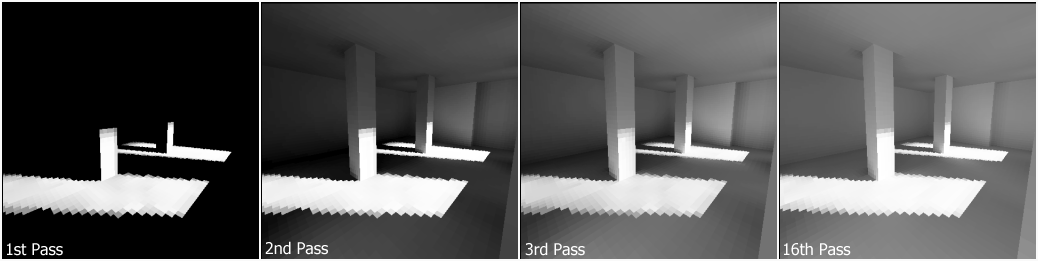
\includegraphics[width=\textwidth]{img/radiosity.png}
	\end{frame}

	\begin{frame}
		\frametitle{Visual effects}
		\begin{columns}
			\column{.6\textwidth}
				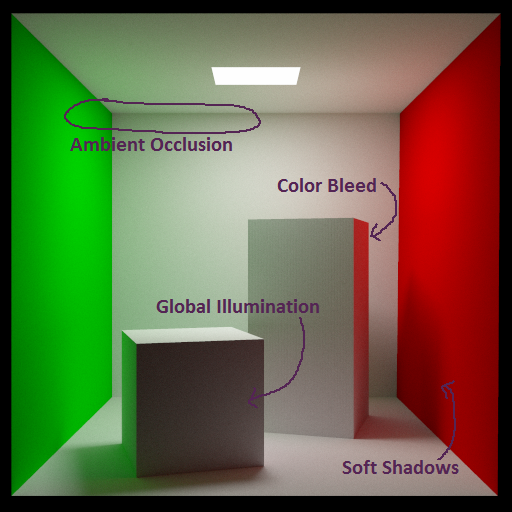
\includegraphics[height=.7\textheight]{img/visual_effects.png}
			\column{.4\textwidth}
				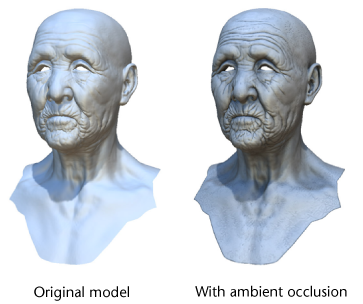
\includegraphics[height=.5\textheight]{img/ambient_occlusion.png}
		\end{columns}
	\end{frame}

	\begin{frame}
		\frametitle{Computational difficulty}
		\begin{itemize}
			\item pathtracing 
				\begin{itemize}
					\item computes multiple ray bounces
					\item requires (hundreds of) thousands of samples 
					\item has to be recomputed if camera or object moves
				\end{itemize}
			\item radiosity
				\begin{itemize}
					\item needs large amount of patches for good results
					\item has to be recomputed if an object moves
				\end{itemize}
			\item tough to be computed in real-time without additional tricks
		\end{itemize}
	\end{frame}

	\begin{frame}
		\frametitle{Traditional rendering}
		\begin{columns}
			\column{.6\textwidth}
				\begin{itemize}
					\item rasterization
					\item way easier to compute than raytracing
					\item interactive framerates
					\item trade-off: not as realistic
					\item requires techniques to simulate visual effects
					\item most of the rendering is done by GPU
					\item abide by rendering pipeline of GPU
				\end{itemize}
			\column{.4\textwidth}
				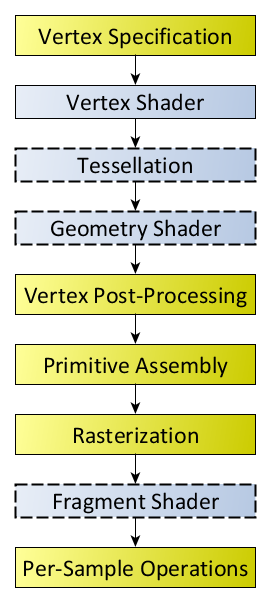
\includegraphics[height=.7\textheight]{img/graphics_pipeline.png}
		\end{columns}
	\end{frame}

	\begin{frame}
		\frametitle{Forward rendering}
		\begin{itemize}
			\item computes geometry and lighting in a single pass:
				\begin{itemize}
					\item for each fragment compute lighting
					\item do z-test (closest fragment for that xy-position?)
					\item if passed, render to frame-buffer, else discard
					\item render frame-buffer to screen
				\end{itemize}
			\item lighting computed regardless if fragment visible or not
			\item however, benefitial for transparency and anti-aliasing
		\end{itemize}
	\end{frame}

	\begin{frame}
		\frametitle{Deferred rendering}
		\begin{columns}
			\column{.6\textwidth}
				\begin{itemize}
					\item computes geometry in first pass:
						\begin{itemize}
							\item albedo-buffer
							\item normal-buffer
							\item z-buffer
						\end{itemize}
					\item render g-buffers to texture-buffer (not screen)
					\item compute lighting in second pass:
						\begin{itemize}
							\item read frontmost geometry from g-buffer
							\item compute lighting
							\item render to screen
						\end{itemize}
					\item only computes lighting for visible fragments
				\end{itemize}
			\column{.4\textwidth}
				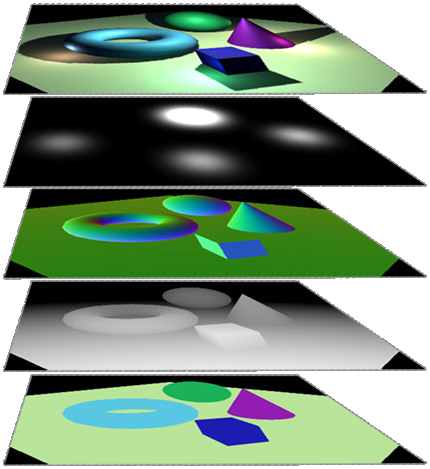
\includegraphics[height=.7\textheight]{img/wiki2_deferred_shading.png}
		\end{columns}
	\end{frame}

	\begin{frame}
		\frametitle{Benefits of deferred rendering}
		\begin{itemize}
			\item forward rendering in $O(objects \cdot lights$):
				\begin{itemize}
					\item for each object
						\begin{itemize}
							\item for each light compute lighting
						\end{itemize}
				\end{itemize}
			\item deferred rendering in $O(objects + lights$):
				\begin{itemize}
					\item for each object
						\begin{itemize}
							\item render geometry
						\end{itemize}
					\item for each light
						\begin{itemize}
							\item compute lighting
						\end{itemize}
				\end{itemize}
			\item lighting computation is way less complex!
			\item we can add way more lights to the scene
		\end{itemize}
	\end{frame}	

	\begin{frame}
		\frametitle{Problems of deferred rendering}
		\begin{itemize}
			\item we \textbf{only} store information about frontmost fragments
			\item but information of deeper layers can improve visual effects
			\item get g-buffers of deeper layers through depth-peeling!
		\end{itemize}
	\end{frame}	

	\begin{frame}
		\frametitle{Depth-peeling}
		\begin{columns}
			\column{.6\textwidth}
				\begin{itemize}
					\item compute first layer g-buffers as usual
					\item for further layers, peel away the previous layers
					\item effectively returns closest-, second-closest, ... n-closest layers
				\end{itemize}
			\column{.4\textwidth}
				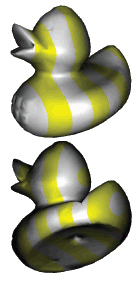
\includegraphics[height=.8\textheight]{img/depth_peeling_duck.png}
		\end{columns}
	\end{frame}	

	\begin{frame}
		\frametitle{Deep G-Buffers}
		\begin{columns}
			\column{.5\textwidth}
				\begin{itemize}
					\item idea: also gather geometry of n-closest layer
					\item generate 2-layer deep g-buffer with depth-peeling or oracle
					\item enforce minimum depth separation
					\item consider second layer for visual effects
				\end{itemize}
			\column{.5\textwidth}
				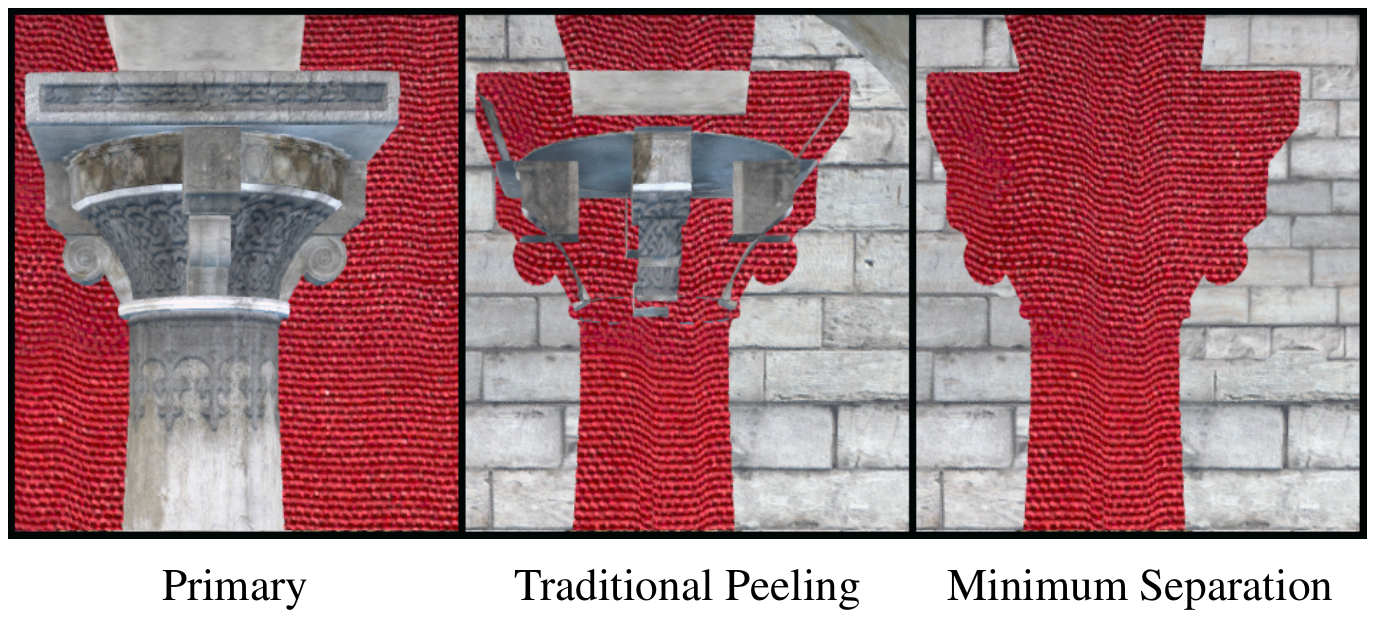
\includegraphics[height=.49\textwidth]{img/minimum_depth_separation.png}
		\end{columns}
	\end{frame}	

	\begin{frame}
		\frametitle{Generating a 2-layer deep g-buffer (depth-peeling)}
		\begin{itemize}
			\item \textbf{depth-peeling method}
			\item collect first layer g-buffer as usual
			\item compute second layer g-buffer by peeling the first layer
			\item takes two passes over scene geometry\pause
			\item instead use oracle and do it in a single pass!
		\end{itemize}
	\end{frame}	

	\begin{frame}
		\frametitle{Generating a 2-layer deep g-buffer}
		\begin{itemize}
			\item \textbf{use some oracle to predict first layer z-buffer}
			\item remember that we are running some simulation/animation
			\item frames are computed per time-step
			\item after a time-step, the object locations won't change \textbf{that much}
			\item we even have knowledge of position and velocity updates
			\item exploit this by recycling information from the previous frame and adjusting it a little
			\item 4 different variants available
			
		\end{itemize}
	\end{frame}	

	\begin{frame}
		\frametitle{Generating a 2-layer deep g-buffer (previous variant)}
		\begin{itemize}
			\item \textbf{previous variant}
			\item recycle first layer z-buffer of previous frame
			\item the smaller the position updates, the smaller the error
			\item even then, errors would only appear in the second layer (invisible unless transparent)
			\item does not guarantee minimum separation
		\end{itemize}
	\end{frame}	

	\begin{frame}
		\frametitle{Generating a 2-layer deep g-buffer (delay variant)}
		\begin{itemize}
			\item \textbf{delay variant}
			\item introduce a frame of latency
			\item frame and animation/simulation are out of sync by one frame
			\item use first layer z-buffer of precomputed latency frame 
			\item drawback: one frame of latency
		\end{itemize}
	\end{frame}	

	\begin{frame}
		\frametitle{Generating a 2-layer deep g-buffer (predict variant)}
		\begin{itemize}
			\item \textbf{predict variant}
			\item use velocities from animation/simulation
			\item predict position updates of objects
			\item 
		\end{itemize}
	\end{frame}	

	\begin{frame}
		\frametitle{Generating a 2-layer deep g-buffer (reproject variant)}
		\begin{itemize}
			\item \textbf{reproject variant}
			\item performs minimum separation test against previous frame's first layer z-buffer
			\item visibility test done using previous z-buffer ("in the past")
			\item same source of error as predict variant, but not as bad (velocities are perfect)
			\item delivers most stables performance out of the 4 variants
			
		\end{itemize}
	\end{frame}	

	\begin{frame}
		\frametitle{Stable global illumination approximation}
		\begin{itemize}
			\item compute screen space ambient occlusion (SSAO) 
			\item compute \textbf{one} radiosity iteration \textbf{per frame}
			\item compute screen space reflections
			\item apply direct and ambient light
		\end{itemize}
	\end{frame}	

	\begin{frame}
		\frametitle{Screen space ambient occlusion}
		\begin{columns}
			\column{.6\textwidth}
				\begin{itemize}
					\item compute ambient occlusion factor $AO$ for \textbf{both layers}
					\item depth discontinuity is now accouted for
					\item results will look more like actual ambient occlusion instead of approximate
				\end{itemize}
			\column{.4\textwidth}
				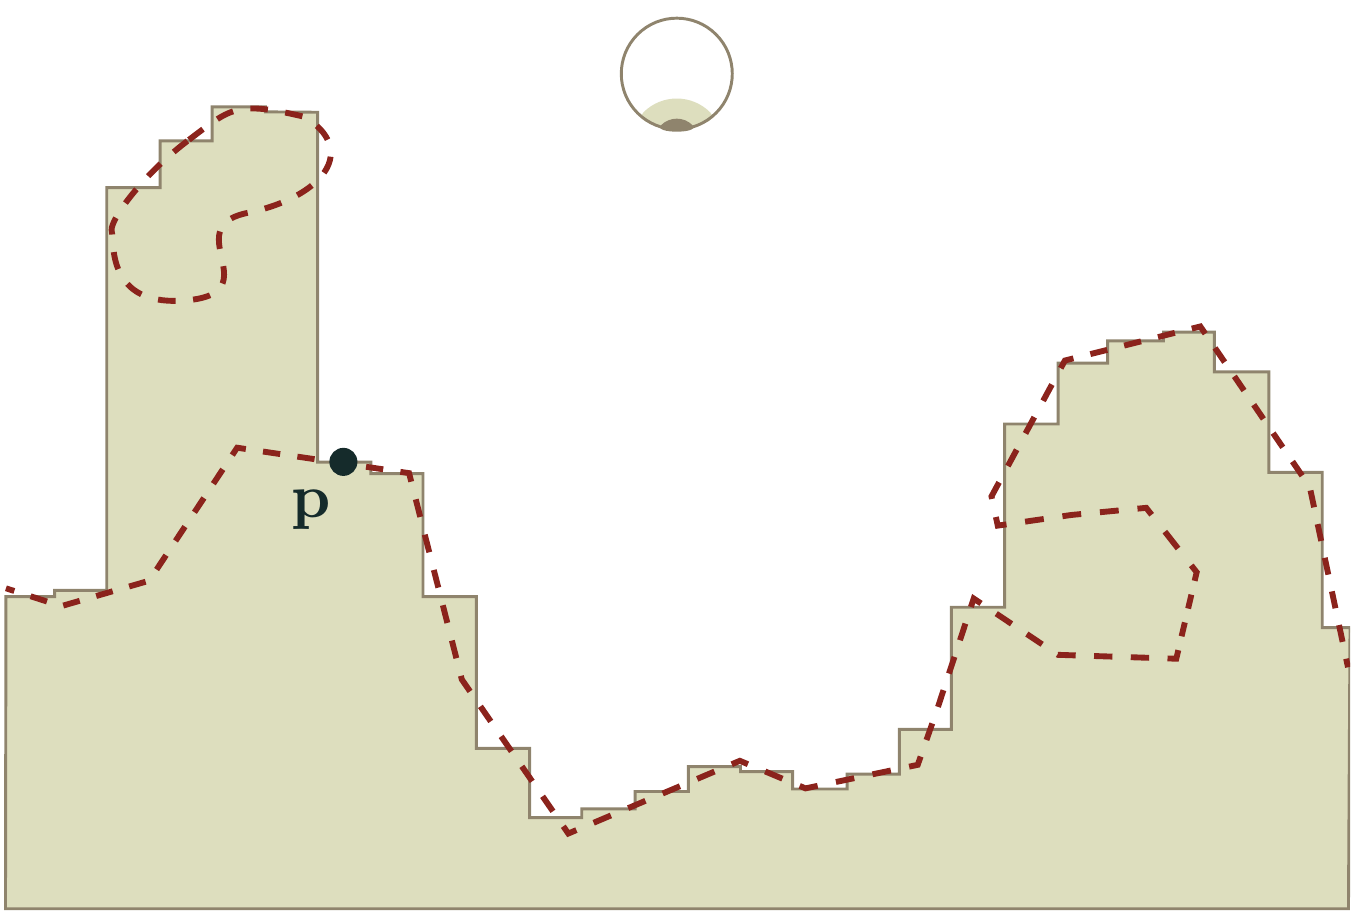
\includegraphics[height=.65\textwidth]{img/ambient_occlusion_depth_discontinuity.png}
				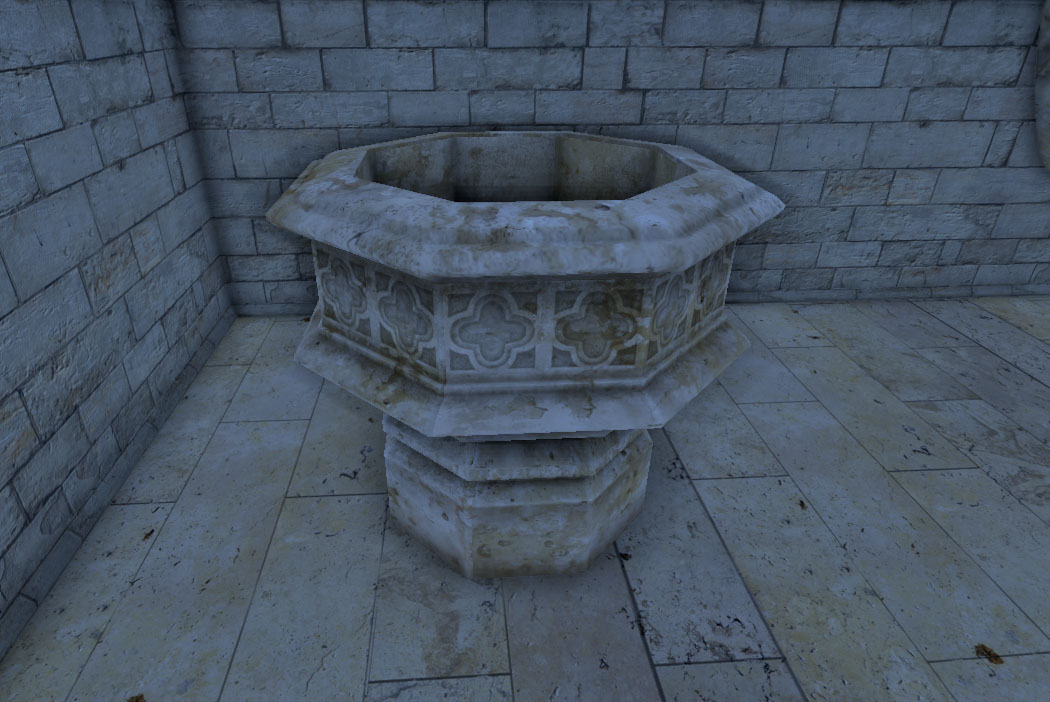
\includegraphics[height=.65\textwidth]{img/screen_space_ambient_occlusion_halo.png}
		\end{columns}		
	\end{frame}	

	\begin{frame}
		\frametitle{Screen space radiosity}
		\begin{itemize}
			\item divide screen space into patches using g-buffers
			\item define form-factor taking into account both g-buffer layers
			\item 
			\item compute \textbf{one} bounce per frame
			\item accumulate bounces from previous frames
			\item ghosting may occur: introduce ways to damp previous lighting
		\end{itemize}
	\end{frame}	

	\begin{frame}
		\frametitle{Screen space mirror reflections}
		\begin{itemize}
			\item march reflection rays in cameraspace
			\item project reflection onto both g-buffers
			\item if distance is within minimum depth separation, it's a hit
			\item else switch to cube-mapping
		\end{itemize}
	\end{frame}	

	\begin{frame}
		\frametitle{Screen space mirror reflections (cube mapping)}
		\begin{itemize}
			\item render scene from 6 angles (cube-like)
			\item march reflection ray
			\item look-up reflection point in cube-map
		\end{itemize}
	\end{frame}	

	\begin{frame}
		\frametitle{Results}
		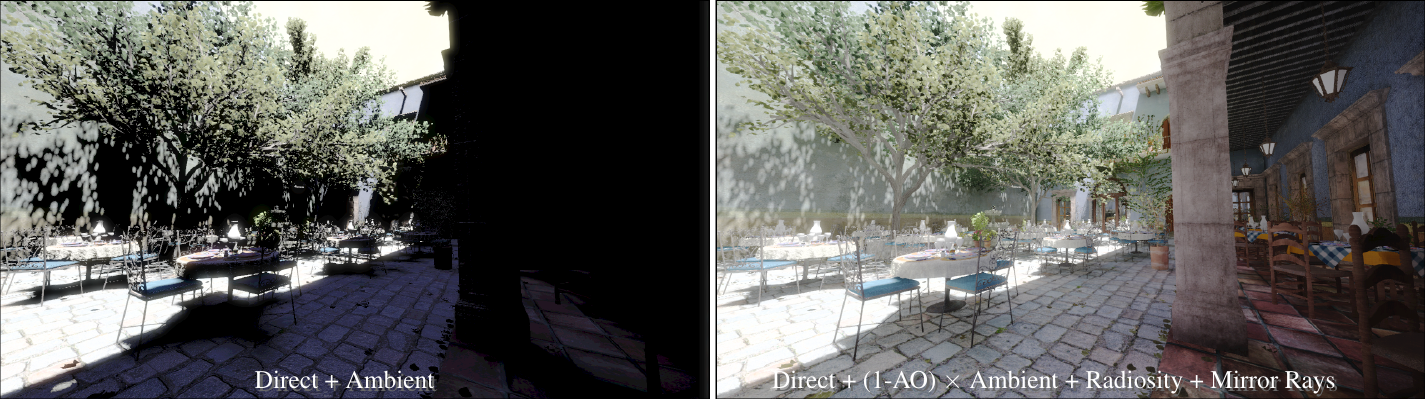
\includegraphics[width=\textwidth]{img/deep_g_buffer_render.png}
		\begin{itemize}
			\item 1920x1080 resolution
			\item rendered using NVIDIA GeForce 980
			\item in 10.8ms (92 FPS)
		\end{itemize}
	\end{frame}

\end{document}